\documentclass[conference]{IEEEtran}
\usepackage{booktabs}
\usepackage{graphicx}
\usepackage{amsmath}
\usepackage{url}
\usepackage[hidelinks]{hyperref}
\graphicspath{{../results/stage4/figures/}{../results/stage4e/figures/}{../results/figures/}}
\newcommand{\pending}{\textit{[pending Stage 4e results]}}

\begin{document}
\title{Reproducing Transfer-Learning Diabetic Retinopathy Grading on APTOS 2019:\\
Ordinal Regression, Imbalance-Aware Losses and a Strict-Protocol Gap Analysis}
\author{\IEEEauthorblockN{Shivansh, Divyanshi, Vivek, Shubham}
\IEEEauthorblockA{CV Research-Reproduction Project --- Diabetic Retinopathy Grading (Final Report)}}
\maketitle

\begin{abstract}
Chilukoti \emph{et al.} (2024) report a quadratic weighted kappa (QWK) of 0.954 on APTOS~2019 with an
ImageNet-initialised EfficientNet-B3, CLAHE pre-processing and a snapshot ensemble, without public code. We
re-implemented the method from the text. With the stated recipe we obtain QWK 0.81--0.82 on a stratified held-out
test set. A lower learning rate and augmentation raise this to 0.898 (10-snapshot vote). We then test one
pre-registered change: replacing five-class cross-entropy with ordinal regression (squared error on the grade,
cut-offs tuned on validation). Over three seeds it raises the ensemble QWK from 0.897 to 0.914, cuts errors of two or
more grades by 26\% and lifts Severe NPDR recall from 0.28 to 0.40. The gain survives a matched soft-vote control
(+0.015, 95\% CI [+0.002, +0.030]), but it appears only in the ensemble and was significant in only one of three
seeds, so our primary prediction was not confirmed. We then test the two strategies from our literature review
that the baseline lacked. Focal loss ties cross-entropy under every decision rule (+0.004). Class-balanced ordinal
regression raises Severe recall from 0.40 to 0.46 at a small QWK cost ($-0.006$), but the gain rests on one of three
seeds. Across all ten arms, tuning the cut-offs on validation matters more than the choice of loss.
Finally, under a strict protocol where every choice is made on validation or out-of-fold data and the test set is
opened once, a 5-fold Noisy-Student EfficientNet ensemble reaches QWK 0.918 [0.900, 0.935]. Choosing cut-offs and
members on the test set reaches only 0.928, and no model exceeds 0.83 accuracy against the paper's 0.942. We argue
that the paper's figure is not reproducible under a clean split. No clinical claims are made.
\end{abstract}

% =====================================================================================================================
\section{Introduction}
Diabetic retinopathy (DR) is a leading cause of preventable vision loss. Screening programmes grade fundus
photographs on a five-step scale, from no DR to proliferative DR (PDR). Convolutional networks fine-tuned from
ImageNet can be trained on public datasets of a few thousand images, such as APTOS~2019~\cite{aptos2019}.

Chilukoti \emph{et al.}~\cite{chilukoti2024} report QWK~\cite{cohen1968kappa} 0.954 on APTOS~2019 with an
EfficientNet-B3~\cite{tan2019efficientnet}, CLAHE~\cite{zuiderveld1994clahe} and a snapshot
ensemble~\cite{huang2017snapshot}. Our literature review (Phase~1) identified three gaps in work of this kind:
class imbalance (Severe NPDR and PDR are 5\% and 8\% of images), evaluation by accuracy alone, and the unused ordinal
structure of the grades. It ended with a research question: \emph{can class-balanced, ordinal-aware learning
improve Severe NPDR and PDR recognition while reducing clinically large grading errors?}

This report covers the whole project. Stage~2 selected the base paper and checked its reproducibility. Stage~3
reproduced it. Stage~4 tested one pre-registered change (ordinal regression). Stage~4e ran the two remaining
strategies from Phase~1 (focal loss, class-balanced ordinal regression). Stages~4b--4d asked how far a strict
protocol can close the gap to 0.954. Our contributions are:
\begin{enumerate}
\item an open re-implementation of the base paper, with a documented reproduction gap and its diagnosis;
\item a pre-registered, single-change test of ordinal regression, with an ablation that separates the loss from the
decision rule, three seeds and paired bootstrap tests;
\item a controlled comparison of the five training strategies proposed in our literature review;
\item a strict-protocol attempt to close the gap, with the test set opened once, and an analysis of what the
remaining gap can and cannot be explained by;
\item an evaluation that reports per-grade recall, large-error counts and referable-DR sensitivity and specificity,
and a failure analysis that includes a sanity check of the saliency maps.
\end{enumerate}
Every stage's predictions were written before its runs. We report each one as it fell.

% =====================================================================================================================
\section{Related work}
\textbf{Transfer learning and ensembles.} Most DR graders fine-tune an ImageNet CNN. Fang \emph{et al.} fine-tuned
19 ImageNet architectures on APTOS and found that everything newer than VGG lies within about 0.01 QWK (best,
ConvNeXt-Tiny, 0.930)~\cite{fang2023imagenet}. Under 5-fold cross-validation, nnMobileNet reports
0.934~\cite{zhu2023nnmobilenet}. SSiT, on a split shaped like ours, reports $0.930\pm0.003$ even with
self-supervised EyePACS pre-training~\cite{huang2022ssit}.

\textbf{Losses.} In a systematic ResNet-50 study on EyePACS, squared-error regression beat cross-entropy by
+0.020 QWK and focal loss by +0.018~\cite{huang2023resnet}. Focal loss~\cite{lin2017focal} down-weights
well-classified examples and is often proposed for class imbalance. Re-weighting the classes is a cheaper
alternative.

\textbf{Label quality.} DR grading has substantial inter-grader disagreement~\cite{krause2018grader}, and APTOS was
graded by a single person per image. This caps the agreement any model can show against the labels.

% =====================================================================================================================
\section{Base paper and reproducibility (Stage 2)}
The paper fine-tunes an ImageNet EfficientNet-B3 with a three-layer head (512--512--5, dropout 0.5/0.25) on images
pre-processed with CLAHE and a Gaussian blur at $300\times300$. It ensembles ten snapshots of one run by majority
vote. Training uses Adam (lr $10^{-3}$, weight decay $10^{-4}$) with gradient clipping at 0.1.

\textbf{Checklist.} There is no public code. The dataset is public: 3,662 images, class counts
1805/370/999/193/295. The method fits a free T4 GPU. The metric is defined. The APTOS split, batch size, loss, epoch
count for APTOS and CLAHE parameters are \emph{not} stated. We use cross-entropy, global-norm clipping at 0.1, CLAHE
with clip 2.0 and $8\times8$ tiles on LAB lightness, a $5\times5$ blur, batch 16, 60 epochs, and a stratified
70/15/15 split (seed 42; 2,562/550/550 images).

\textbf{Red flags.} In the paper's Table~3, precision, recall and QWK are all exactly 0.867. Constant predictors report
a macro AUC of 0.196, where a constant predictor gives 0.5. Recomputing QWK from the paper's own EyePACS confusion
matrices does not give the reported values. We therefore treat 0.954 as a claim to test.

% =====================================================================================================================
\section{Reproduction (Stage 3)}
\textbf{Duplicates.} Hashing the raw files shows 123 groups of byte-identical images, 30 of them with conflicting
grades. Under our split, 29 of the 550 test images (5.3\%) have a copy in training. Removing them changes QWK by at
most 0.007 in every stage, so the leak does not inflate our scores.

\begin{table}[t]
\centering
\caption{Stage 3 test results (300\,px, 60 epochs, one run each). ``Single'' is the best-validation epoch; ``vote''
is the 10-snapshot majority vote.}
\label{tab:stage3}
\small
\setlength{\tabcolsep}{3pt}
\begin{tabular}{@{}lcc@{}}
\toprule
Setting & QWK single / vote & Sev. / PDR recall (vote) \\
\midrule
Paper (reported) & 0.954 & -- \\
Paper recipe (lr $10^{-3}$) & 0.824 / 0.813 & -- \\
lr $10^{-4}$ & 0.846 / 0.884 & -- \\
\textbf{lr $10^{-4}$ + aug.} & \textbf{0.908 / 0.898} & 0.28 / 0.59 \\
\quad + retina crop & 0.883 / 0.893 & 0.24 / 0.57 \\
\quad + weighted CE & 0.878 / 0.897 & \textbf{0.48} / 0.55 \\
\quad + cosine decay & 0.906 / 0.883 & 0.28 / 0.52 \\
\bottomrule
\end{tabular}
\end{table}

\textbf{Results} (Table~\ref{tab:stage3}). The paper's recipe gives QWK 0.81--0.82. At lr $10^{-3}$, validation QWK
repeatedly collapses and Severe NPDR is never predicted. In this regime the snapshot vote \emph{lowers} QWK, because
the snapshots are uneven. A learning rate of $10^{-4}$ plus flip and rotation augmentation gives 0.908 / 0.898. This
is our baseline. Retina cropping and cosine decay did not help. Class weighting raised Severe recall from 0.28 to 0.48
at the cost of Moderate recall, and QWK did not move. Every lr-$10^{-4}$ variant lies within the bootstrap interval of
the others (about $\pm0.03$). The model \emph{ranks} severity well (macro AUC 0.94) but \emph{decides} poorly
(macro-F1 0.65), and its errors concentrate between neighbouring grades.

% =====================================================================================================================
\section{Hypothesis and method (Stage 4)}
\textbf{Hypothesis.} Cross-entropy treats the five grades as unordered: calling a Severe case No DR costs the same as
calling it PDR. QWK, and the clinic, do not see these mistakes as equal. We replace the five-way output with
\emph{ordinal regression}: one output, trained with mean-squared error against the grade, decoded with four cut-offs
tuned on the validation set. An error of $d$ grades then costs $d^2$, which mirrors the quadratic weights inside QWK.
The tuned cut-offs handle class imbalance without re-weighting.

\textbf{Ablation.} The loss and the decision rule are separated into four arms. Each one decodes the same trained
models (seeds 42, 43, 44, plus one de-duplicated pair):
A, cross-entropy with the paper's majority vote (baseline);
B, cross-entropy with the expected grade and tuned cut-offs;
C, MSE with rounding;
D, MSE with tuned cut-offs (the hypothesis).
Cut-offs are found by coordinate search on validation QWK. The test set never influences a choice.

\textbf{Pre-registered predictions} (ensemble, mean over seeds):
P1, D$-$A of +0.01 to +0.03, with a paired-bootstrap interval excluding 0 in at least 2 of 3 seeds;
P2, errors of $\ge2$ grades fall by at least 25\%;
P3, Severe recall rises by at least 10 points;
P4, PDR recall falls (risk);
P5, referable-DR AUC changes by at most 0.01;
P6, B$-$A is less than half of D$-$A;
P7, C$>$A;
P8, same sign of D$-$A on de-duplicated data.

% =====================================================================================================================
\section{Results: ordinal regression}
\begin{table}[t]
\centering
\caption{Stage 4, 10-snapshot ensemble, mean over 3 seeds (QWK $\pm$ std). Sev./PDR: recall. $\ge$2: errors of two
or more grades (of 550). Sens./Spec.: referable DR (grade $\ge2$).}
\label{tab:stage4}
\small
\setlength{\tabcolsep}{3pt}
\begin{tabular}{@{}lccccc@{}}
\toprule
Arm & QWK & Sev. & PDR & $\ge$2 & Sens./Spec. \\
\midrule
A: CE, vote & $0.897\pm.004$ & 0.28 & 0.61 & 21.7 & .946/.904 \\
A$_\text{soft}$: CE, averaged & $0.899\pm.001$ & 0.25 & 0.61 & 21.3 & -- \\
B: CE, tuned & $0.907\pm.007$ & 0.44 & 0.57 & 15.7 & .982/.879 \\
C: MSE, rounding & $0.896\pm.001$ & 0.47 & 0.17 & 17.0 & .900/.948 \\
\textbf{D: MSE, tuned} & $\mathbf{0.914\pm.004}$ & 0.40 & 0.58 & 16.0 & .963/.909 \\
\bottomrule
\end{tabular}
\end{table}

Table~\ref{tab:stage4} gives the main result. D is the best Stage~4 arm. Five of eight predictions were confirmed:
P2 (errors $\ge2$: $-26\%$), P3 (Severe +12.6 points), P4 (PDR $-3$ points), P5 and P8. The central prediction
\textbf{P1 was not confirmed}. D$-$A is +0.016, inside the predicted range and positive in every seed and on
de-duplicated data. But its interval excludes 0 in only one of three seeds
(+0.012 [$-$0.003, +0.030], +0.023 [+0.006, +0.045], +0.013 [$-$0.006, +0.033]). P6 failed by 0.001 and P7 failed.

\textbf{Neither part works alone.} With rounding, the ordinal model ties the baseline (C$-$A $=-0.001$). PDR recall
collapses to 0.17 because squared error on imbalanced, noisy labels shrinks predictions towards the mean grade. The
tuned top cut-off sits about 0.6 grades below rounding's 3.5 in every seed. The cut-offs undo this shrinkage
(D$-$C $=+0.018$ [+0.007, +0.029], pooled over seeds).

\textbf{Votes vs.\ averages (post-hoc).} Arm A votes while D averages, so part of D$-$A could come from the ensemble
rule rather than the loss. A matched control, A$_\text{soft}$ (averaged probabilities, arg-max), ties A
(+0.001 [$-$0.002, +0.006]). D$-$A$_\text{soft}$ is +0.015 [+0.002, +0.030], pooled over seeds. The gain comes from
the loss and the decision rule together, not from averaging. It still appears \emph{only in the ensemble}: as single
models, all arms tie at about 0.90 (D$-$A $=+0.002$).

\textbf{Trade-off.} D trades accuracy (0.828$\to$0.804) for QWK. It makes fewer far errors and more one-grade errors
(e.g.\ Severe$\to$Moderate falls from 15 to 7, Moderate$\to$Severe rises from 5 to 19, seed 42). For screening this
means higher referable sensitivity (0.946$\to$0.963) at the same specificity.

% =====================================================================================================================
\section{Imbalance-aware losses (Stage 4e)}
\label{sec:stage4e}
Phase~1 proposed five strategies. Stages 3 and 4 tested cross-entropy, weighted cross-entropy and ordinal MSE, but
not \emph{focal loss} or \emph{class-balanced ordinal regression}. Stage~4e runs both under the Stage~4 protocol
(same split, seeds, recipe and decision rules). Only the loss changes:
\begin{itemize}
\item \textbf{Focal loss}~\cite{lin2017focal}, $-(1-p_t)^{\gamma}\log p_t$ with $\gamma=2$ and no $\alpha$, decoded
as E$_\text{vote}$ (like A), E$_\text{soft}$ (like A$_\text{soft}$) and E$_\text{tuned}$ (like B).
\item \textbf{Class-balanced MSE}, $w_c\,(\hat y-y)^2$ with $w_c\propto n_c^{-1/2}$, normalised to mean 1 (weights
0.69, 1.53, 0.93, 2.12, 1.71 for grades 0--4; the Stage~3 weighted-CE weights), decoded as F$_\text{round}$ (like C)
and F$_\text{tuned}$ (like D).
\end{itemize}
The Stage~4 models are reused. Two Stage~4 runs were retrained on the new platform (Kaggle) as a control. The
predictions (Q1--Q8, Table~\ref{tab:stage4e_pred}) were fixed before any run and are recorded in the first
version of the Kaggle kernels. Stage~4e ran after the test set
had been opened in Stage~4c (Sec.~\ref{sec:strict}), so its test numbers are post-test and drive no choice.

\IfFileExists{generated/stage4e_table.tex}{\begin{table}[t]
\centering
\caption{Stage 4e (post-test) with the Stage 4 arms, 10-snapshot ensemble, mean over seeds. CB-MSE: class-balanced MSE. Columns as in Table~\ref{tab:stage4}.}
\label{tab:stage4e}
\footnotesize
\setlength{\tabcolsep}{2.5pt}
\begin{tabular}{@{}lccccc@{}}
\toprule
Arm & QWK & Sev. & PDR & $\ge$2 & Sens./Spec. \\
\midrule
A: CE, vote & $0.897\pm.004$ & 0.28 & 0.61 & 21.7 & .946/.904 \\
A$_\text{soft}$: CE, averaged & $0.899\pm.001$ & 0.25 & 0.61 & 21.3 & .949/.904 \\
B: CE, tuned & $0.907\pm.007$ & 0.44 & 0.57 & 15.7 & .982/.879 \\
\midrule
E$_\text{vote}$: focal, vote & $0.901\pm.004$ & 0.24 & 0.58 & 21.0 & .945/.914 \\
E$_\text{soft}$: focal, averaged & $0.903\pm.001$ & 0.23 & 0.60 & 20.7 & .948/.915 \\
E$_\text{tuned}$: focal, tuned & $0.911\pm.003$ & 0.54 & 0.53 & 10.0 & .982/.889 \\
\midrule
C: MSE, rounding & $0.896\pm.001$ & 0.47 & 0.17 & 17.0 & .900/.948 \\
D: MSE, tuned & $0.914\pm.004$ & 0.40 & 0.58 & 16.0 & .963/.909 \\
\midrule
F$_\text{round}$: CB-MSE, rounding & $0.888\pm.011$ & 0.45 & 0.22 & 18.0 & .873/.956 \\
F$_\text{tuned}$: CB-MSE, tuned & $0.908\pm.001$ & 0.46 & 0.55 & 16.0 & .943/.915 \\
\bottomrule
\end{tabular}
\end{table}
}{\noindent Results table \pending.}

\IfFileExists{generated/stage4e_predictions.tex}{\begin{table}[t]
\centering
\caption{Stage 4e predictions (fixed before the runs) and pooled paired-bootstrap contrasts (ensemble, mean over seeds, 95\% CI).}
\label{tab:stage4e_pred}
\footnotesize
\setlength{\tabcolsep}{2pt}
\begin{tabular}{@{}p{0.07\columnwidth}p{0.5\columnwidth}p{0.3\columnwidth}c@{}}
\toprule
\# & Prediction & Observed & OK? \\
\midrule
Q1 & focal does not change QWK under the same rule & E$_\text{vote}$ $-$ A +0.004; E$_\text{tuned}$ $-$ B +0.004 & yes \\
Q2 & focal raises Severe recall under the vote by $\ge$ 0.05 & 0.276 $\to$ 0.241 & \textbf{no} \\
Q3 & ordinal still beats focal (D $>$ E$_\text{tuned}$) & D $-$ E$_\text{tuned}$ +0.003 & yes$^a$ \\
Q4 & class balancing raises Severe recall on top of ordinal by $\ge$ 0.05 & 0.402 $\to$ 0.460 & yes$^b$ \\
Q5 & class balancing costs no QWK ($|$F$_\text{tuned}$ $-$ D$|$ $<$ 0.01) & F$_\text{tuned}$ $-$ D $-$0.006 & yes \\
Q6 & errors $\ge$ 2 grades do not rise by more than 10\% & 16.0 $\to$ 16.0 & yes \\
Q7 & class balancing lifts PDR recall under rounding by $\ge$ 0.15 & 0.167 $\to$ 0.220 & \textbf{no} \\
Q8 & sanity: Kaggle controls within 0.015 of Colab (A, D) & A +0.011; D $-$0.002 & yes \\
\midrule
\multicolumn{4}{@{}l}{\textit{Contrast: $\Delta$QWK [95\% CI]}} \\
\multicolumn{4}{@{}l}{E$_\text{vote}$ $-$ A: $+0.004$ [$-0.003$, $+0.011$]} \\
\multicolumn{4}{@{}l}{E$_\text{soft}$ $-$ A$_\text{soft}$: $+0.004$ [$-0.003$, $+0.012$]} \\
\multicolumn{4}{@{}l}{E$_\text{tuned}$ $-$ B: $+0.004$ [$-0.003$, $+0.013$]} \\
\multicolumn{4}{@{}l}{D $-$ E$_\text{tuned}$: $+0.003$ [$-0.007$, $+0.012$]} \\
\multicolumn{4}{@{}l}{F$_\text{tuned}$ $-$ D: $-0.006$ [$-0.014$, $+0.000$]} \\
\multicolumn{4}{@{}l}{F$_\text{round}$ $-$ C: $-0.008$ [$-0.018$, $-0.001$]} \\
\multicolumn{4}{@{}l}{F$_\text{tuned}$ $-$ A: $+0.010$ [$-0.005$, $+0.026$]} \\
\bottomrule
\end{tabular}
\par\vspace{2pt}\parbox{\columnwidth}{\footnotesize $^a$In sign only; the CI includes 0. $^b$On the mean only; per seed the gain is 0, +0.17 and 0 (five images in one seed).}
\end{table}
}{\noindent Prediction check \pending.}

\IfFileExists{sections/stage4e_discussion.tex}{% Stage 4e discussion, written from ../results/stage4e (see ../stage4e_results.md).
\textbf{Focal loss changes nothing under the paper's rule.} Focal ties cross-entropy under the vote (+0.004),
averaging (+0.004) and tuned cut-offs (+0.004), and no interval excludes 0 (Q1). Under the vote, Severe recall
falls rather than rises (0.28$\to$0.24, Q2 fails). This agrees with the +0.003 reported for focal loss on
EyePACS~\cite{huang2023resnet}.

\textbf{Class balancing gives a small, unstable gain in Severe recall.} With tuned cut-offs, class-balanced MSE
raises mean Severe recall from 0.40 to 0.46 at an unchanged count of large errors (Q4, Q6). The gain comes from one
seed, however: per seed it is 0, +0.17 and 0, which is five extra Severe images in seed~43. QWK falls in all three
seeds ($-0.006$, CI $[-0.014, +0.000]$), so Q5 holds only narrowly, and referable sensitivity drops from 0.963 to
0.943. With plain rounding, the weights do not undo the shrinkage of the regression output: PDR recall moves only
from 0.17 to 0.22, and QWK falls ($-0.008$, CI excludes 0; Q7 fails).

\textbf{The decision rule matters more than the loss.} The four arms with validation-tuned cut-offs (B, D,
E$_\text{tuned}$, F$_\text{tuned}$) reach 0.907--0.914. The six arms with a vote, averaging or rounding reach
0.888--0.903. Among the tuned arms, the loss moves QWK by at most 0.007.

\textbf{Platform control.} The Kaggle re-runs of seed~42 land within 0.015 of Colab (Q8): D moves by $-0.002$ and
A by $+0.011$. Against the same-platform controls, focal is lower than cross-entropy (0.896 vs.\ 0.908), and
F$_\text{tuned}$ ties D (0.908 vs.\ 0.908). Both readings agree with the pooled contrasts.

\textbf{Answer to the Phase~1 question.} By the reading rule fixed in the plan, class-balanced ordinal learning
improves Severe NPDR recall at no significant QWK cost. Because the gain rests on five images in one seed and costs
referable sensitivity, we keep ordinal regression with tuned cut-offs (D) as our recommended strategy. Class
balancing remains an optional trade toward Severe recall.

\textbf{An unplanned observation.} Focal loss with tuned cut-offs makes the fewest errors of two or more grades in
every seed (9, 10, 11, against 15--18 for B, D and F$_\text{tuned}$). It also has the highest Severe recall (0.54),
at the cost of Moderate recall (0.64 vs.\ 0.80 for D). This was not predicted and was seen after the test set was
opened, so it is a lead for future work, not a result.
}{}

% =====================================================================================================================
\section{Closing the gap under a strict protocol (Stages 4b--4d)}
\label{sec:strict}
Stage~4 left a gap of 0.04 to the paper. Stages~4b--4c asked how much of it a stronger recipe can close when
\emph{every} choice is made on validation or out-of-fold (OOF) predictions and the test set is opened once, after
all training. On 5-fold cross-validation over the 3,112 train+val images, the levers adopted were peak lr
$3\times10^{-4}$ (+0.017 validation QWK), strong augmentation (+0.013), label cleaning (+0.010), Ben Graham
pre-processing~\cite{graham2015} (+0.014), Noisy-Student EfficientNet-B4 weights~\cite{xie2020noisy}, higher
resolution (380--512\,px) and 5-fold ensembles. Thirty epochs instead of 60 was rejected ($-0.006$). Diverse members
were added greedily by OOF gain: ConvNeXt-Tiny, SE-ResNeXt50, a retina-crop B4, B4 at 512\,px and B4 after five
epochs of EyePACS-2015 pre-training (external data, never in the headline). Only B4 at 512\,px was selected.

\begin{table}[t]
\centering
\caption{Strict protocol, test set (550 images) opened once. Rows in italics choose on the test set and are not
results.}
\label{tab:strict}
\small
\setlength{\tabcolsep}{3pt}
\begin{tabular}{@{}lcc@{}}
\toprule
Model & Test QWK [95\% CI] & Acc. \\
\midrule
Stage 4 A (seed 42) & 0.898 [0.868, 0.921] & 0.829 \\
Stage 4 D (seed 42) & 0.910 [0.887, 0.929] & 0.802 \\
4b: B4-NS 380 + B3 384 & 0.916 [0.896, 0.932] & 0.802 \\
\textbf{4c: + B4-NS 512} & \textbf{0.918 [0.900, 0.935]} & 0.807 \\
\textit{cut-offs tuned on test} & \textit{0.924} & \textit{0.827} \\
\textit{best of 63 subsets + cut-offs on test} & \textit{0.928} & \textit{0.791} \\
Paper (reported) & 0.954 & 0.942 \\
\bottomrule
\end{tabular}
\end{table}

\textbf{Result} (Table~\ref{tab:strict}). The headline is 0.918 [0.900, 0.935] (OOF 0.928), against Stage~4 A
+0.020 [+0.001, +0.042]. The paper's 0.954 lies outside the interval. Four of seven Stage~4c predictions held.
Architecture diversity, EyePACS pre-training and the optimistic rows did not. A post-test Stage~4d re-ran the EyePACS
arm with a low fine-tune learning rate. The mid-training dip disappeared, but the final OOF was lower (0.906 vs.\
0.913 originally and 0.920 from ImageNet), so the learning-rate explanation was rejected.

\textbf{What cannot explain the gap.} Choosing cut-offs, members and subsets on the test set lifts our blend to
0.928 at most. Test images with a training twin do not inflate scores. A favourable draw of the split could add
roughly 0.01--0.02. Even stacked, these fall short of 0.954. More tellingly, every selection effect leaves accuracy
between 0.79 and 0.83, against the paper's 0.942. Our 0.928 OOF already sits at the published strict ceiling
(0.92--0.934)~\cite{fang2023imagenet,zhu2023nnmobilenet,huang2022ssit}. A literature-based estimate puts every
remaining strict lever at no more than +0.004 OOF each, below what our test set can detect (about 0.007--0.018 at
80\% power). The explanations left are a reporting error (the paper's EyePACS tables fail their own arithmetic) or an
evaluation set that overlaps training, for example a split made after offline augmentation.

% =====================================================================================================================
\section{Failure analysis}
\IfFileExists{../results/stage4e/figures/gradcam_retina.png}{%
\begin{figure*}[t]
\centering
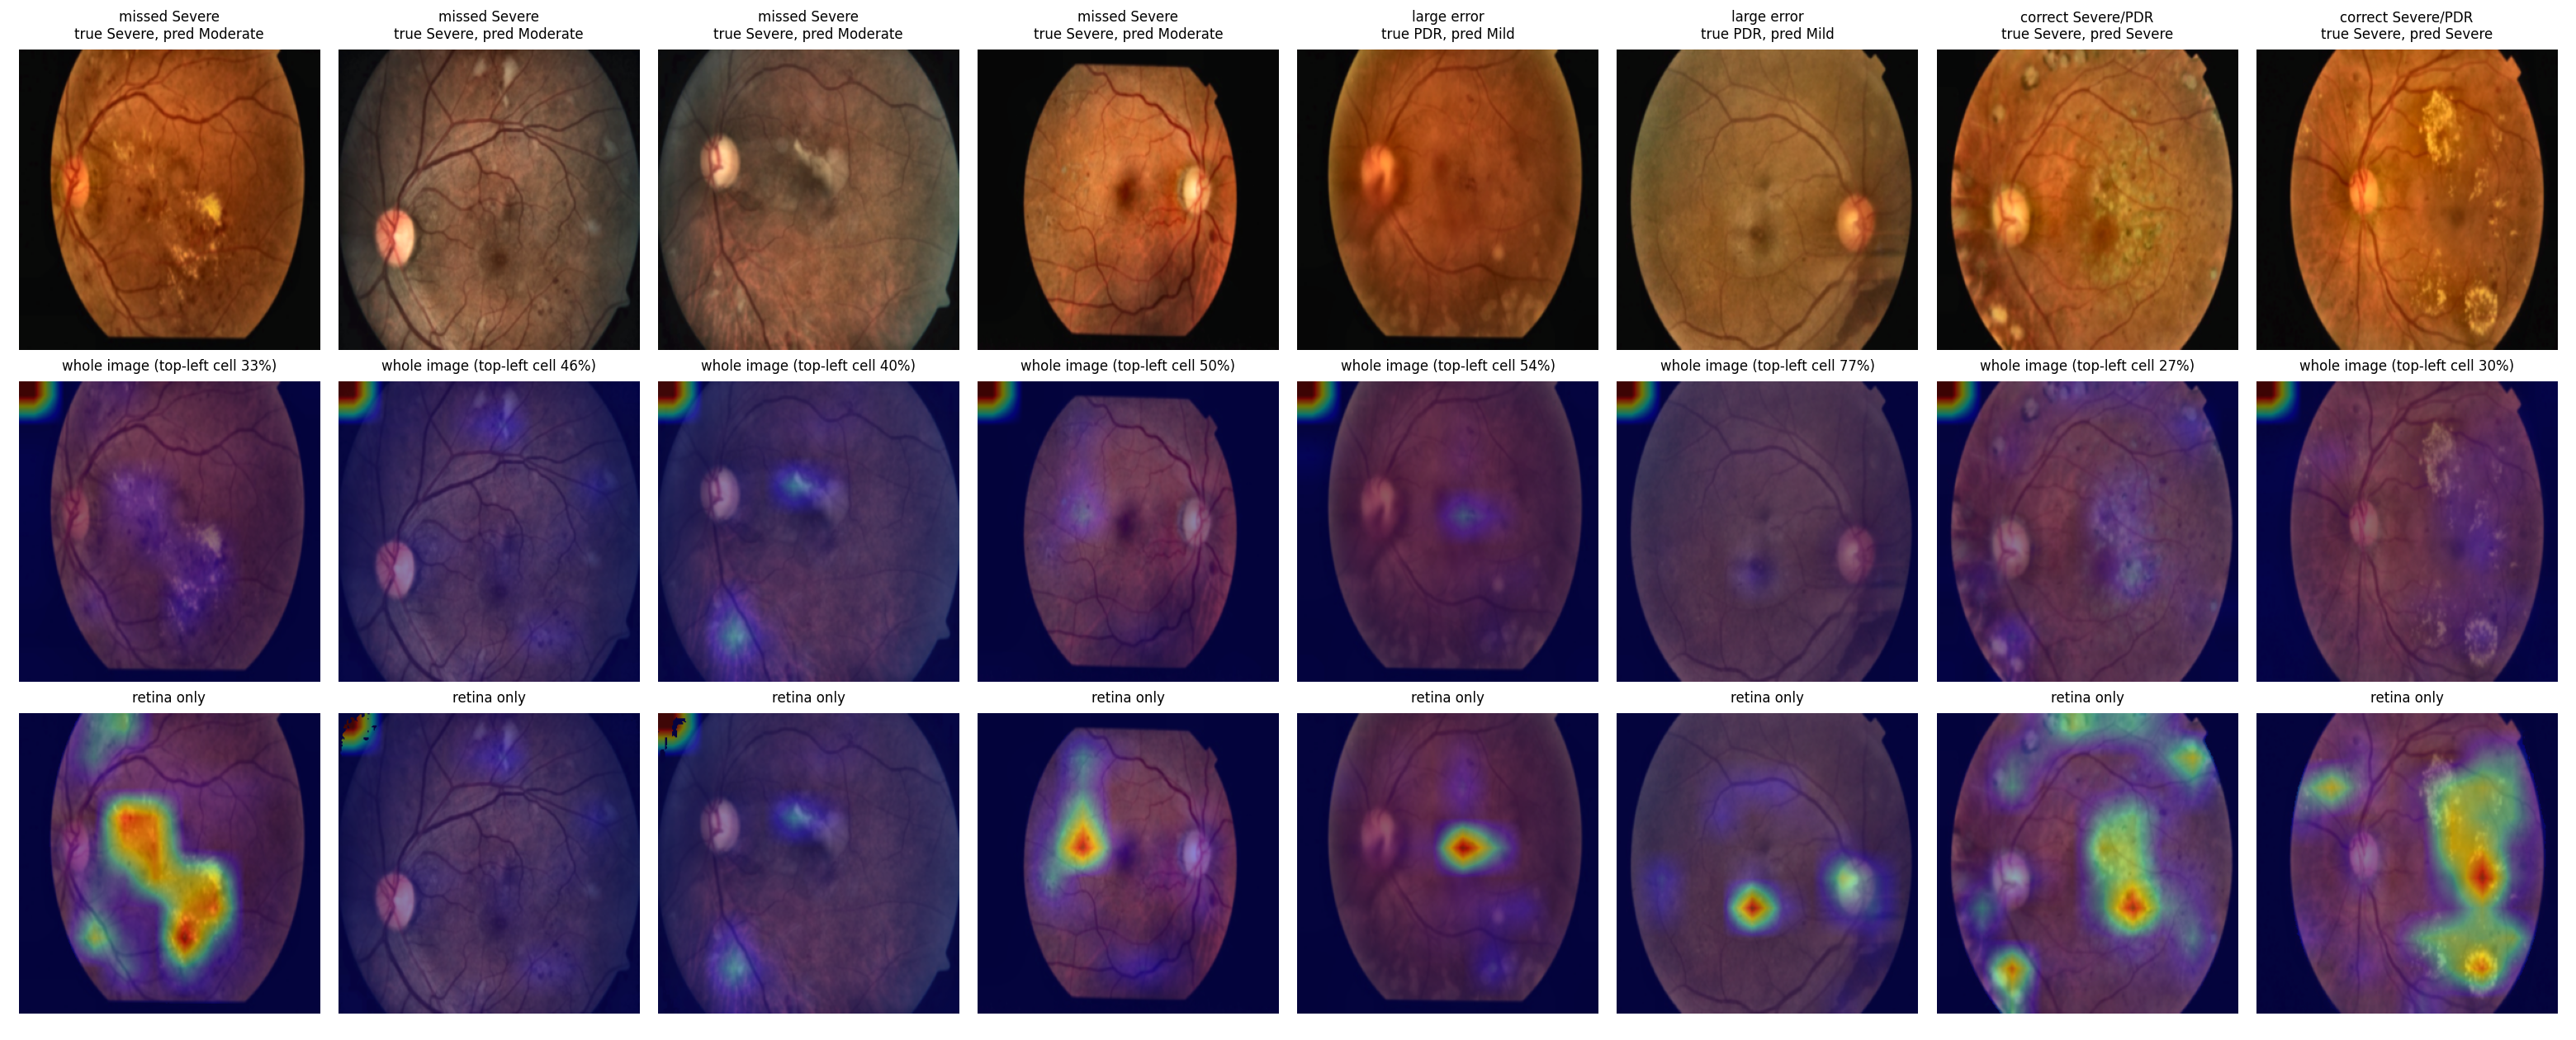
\includegraphics[width=\textwidth]{gradcam_retina.png}
\caption{Grad-CAM for the ordinal model of seed~42 (best-validation weights, 300\,px) on four missed Severe cases, two PDR images graded Mild and two
correct Severe cases. Top: input. Middle: raw map, dominated by the top-left padding cell (share given above each
panel). Bottom: map restricted to feature cells inside the retina. Qualitative only.}
\label{fig:gradcam}
\end{figure*}}{}
\textbf{Label noise sets a floor.} Seven test images belong to identical-image groups with conflicting grades. Arms A
and D both get 6 of the 7 wrong (86\%), against 16--19\% on the other images.

\textbf{Errors concentrate in poorer photos.} For arm D (seed 42), misgraded images are blurrier than correctly
graded ones: median Laplacian variance 50.9 vs.\ 62.8, Mann-Whitney $p=0.0005$, $n=109$ vs.\ 441. They are also
slightly darker (87.8 vs.\ 92.9, $p=0.046$).

\textbf{Saliency maps need a sanity check.} Our first Grad-CAM~\cite{selvaraju2017gradcam} figure peaked in the black
top-left corner for every image, right or wrong. At 300\,px, EfficientNet-B3's stride-2 convolutions pad only the
top and left edges. The top-left cell of the $10\times10$ feature map is then 30--45$\times$ stronger than the median
cell, even for a uniform grey image. \IfFileExists{generated/gradcam_share.tex}{For the 8 images we inspected, that single cell holds 27\%--77\% of the raw map (median 46\%).
}{}
After masking feature cells outside the retina, the corner peak disappears in 6 of the 8 images, and the warm areas
fall on lesions such as exudates (Fig.~\ref{fig:gradcam}). In the other two, the fundus fills the frame, so the corner
cell lies inside the mask. These maps remain qualitative. Read as explanations without the sanity check, they would have been wrong~\cite{adebayo2018sanity}.

\textbf{Remaining confusions are between neighbours}: Mild/Moderate, Moderate/Severe, and PDR called Moderate. These
boundaries depend on counting lesions and seeing new vessels, which is hard at 300\,px.

% =====================================================================================================================
\section{Limitations}
One dataset, one split and no external validation. Three seeds give only a rough view of training noise, and the
bootstrap intervals cover test-set noise only. The test set holds 29 Severe and 44 PDR images, so one image is 3.4
points of Severe recall. Cut-offs are tuned on 550 validation images and move by up to 0.6 between seeds. Several
paper details were assumed. Stage~4e ran on a different platform from Stage~4 (controlled by two retrained runs) and
after the test set had been opened. EyePACS was tried only as five epochs of pre-training, so the paper's 0.967 with
EyePACS remains out of scope. \textbf{No clinical claims are made:} agreement with one grader's labels on a curated
competition set says nothing about screening performance.

% =====================================================================================================================
\section{Conclusion}
The paper's stated recipe gives QWK 0.81--0.82 on a clean split, not 0.954. A lower learning rate and augmentation
reach 0.90. Ordinal regression with validation-tuned cut-offs adds a consistent +0.015--0.016 in the ensemble and
reduces far errors and missed Severe cases, but it fell short of our own pre-registered significance criterion. The
best strict-protocol model reaches 0.918 [0.900, 0.935], at the published ceiling for ImageNet-only training. The
remaining gap, especially in accuracy, is not explained by any protocol choice we could measure. On our Phase~1
question, focal loss brings nothing over cross-entropy. Class-balanced ordinal regression trades a little QWK for
Severe recall, but the gain is unstable across seeds. What moves QWK is the decision rule: every arm with
validation-tuned cut-offs beats every arm without them. Our recommended strategy remains ordinal regression with
tuned cut-offs.

\textbf{Reproducibility.} All notebooks, Kaggle kernel builders, plans with predictions, raw outputs and result tables
are in the project repository. Each stage's plan and predictions were written before its runs.

\bibliographystyle{IEEEtran}
\bibliography{final_refs}
\end{document}
